\chapter{Storytelling and Dashboard Design}

Data analysis is not just about crunching numbers; it is about uncovering stories hidden within the data. In this chapter, we explore how to bring data to life through storytelling and dashboards, enabling both technical and non-technical audiences to understand insights quickly and interactively.

\section*{What is Data Storytelling?}

Data storytelling is the art of communicating data-driven insights in a compelling and relatable manner. It blends three critical elements:

\begin{itemize}
    \item \textbf{Data:} The foundation of your story, extracted through analysis.
    \item \textbf{Narrative:} A structured storyline that explains what the data shows and why it matters.
    \item \textbf{Visuals:} Graphs, charts, and dashboards that enhance understanding.
\end{itemize}

\textbf{Example:} Imagine analyzing temperature and precipitation data for a region. The raw data reveals seasonal patterns. A story might describe how monsoon months show increased rainfall and how rising temperatures correlate with dry spells. These patterns, when shown visually, become easier to interpret and act upon.

\subsection*{Key Elements of a Good Data Story}
\begin{itemize}
    \item \textbf{Context:} Why should we care about this data?
    \item \textbf{Conflict:} What trends or anomalies are surprising or concerning?
    \item \textbf{Conclusion:} What action or insight can be derived?
\end{itemize}

\section{Introduction: Packages and Tools}

In data analysis, storytelling and dashboard creation are essential to communicate insights effectively. While raw data and statistical results are important, they often need to be presented visually to engage the audience and support decision-making.

This section introduces some of the popular tools and software packages widely used for storytelling through infographics and building interactive dashboards. These tools vary in complexity and purpose, ranging from simple graphic design platforms to advanced data visualization libraries.

\subsection*{R Packages}

R offers a rich ecosystem of packages for data visualization and interactive dashboards. Notable examples include:

\begin{itemize}
    \item \textbf{ggplot2} — a versatile and powerful plotting package for creating static and dynamic visualizations.
    \item \textbf{plotly} — adds interactivity to plots made with ggplot2 and supports standalone interactive charts.
    \item \textbf{shiny} — a framework for building fully interactive web applications and dashboards directly from R.
    \item \textbf{flexdashboard} — simplifies creating dashboards using R Markdown.
\end{itemize}

\subsection*{Python Libraries}

Python also provides a range of libraries for storytelling and dashboards, such as:

\begin{itemize}
    \item \textbf{matplotlib} and \textbf{seaborn} for static visualizations.
    \item \textbf{plotly} and \textbf{bokeh} for interactive plots.
    \item \textbf{Dash} — a framework to build interactive dashboards using Python.
\end{itemize}

\subsection*{Graphic Design Tools}

For designing infographic posters and visual storytelling, tools like:

\begin{itemize}
    \item \textbf{Canva} — a user-friendly online design platform with ready-made templates suitable for infographics and reports.
    \item \textbf{Adobe Illustrator} and \textbf{Photoshop} — professional tools for custom and detailed graphic design.
\end{itemize}

\subsection*{Dashboard Platforms}

Dedicated dashboard platforms allow integration of data sources and creation of dynamic dashboards without coding:

\begin{itemize}
    \item \textbf{Tableau} — widely used for interactive, drag-and-drop dashboards.
    \item \textbf{Power BI} — Microsoft’s business analytics tool for interactive visualizations.
    \item \textbf{Google Data Studio} — a free tool for creating reports and dashboards with Google data integration.
\end{itemize}

% \begin{figure}[H]
% \centering
% \includegraphics[width=0.9\textwidth]{dashboard_comparison.png}
% \caption{Comparison of Dashboard Tools and Design Platforms}
% \end{figure}


\section{Infographic Posters}

Infographic posters are a creative way to turn complex data into simple, engaging visuals. By using graphics, key facts, and clear messages, they help people quickly understand important information. Whether for students, professionals, or the general public, these posters make it easier to connect with the audience, spark interest, and improve understanding and memory.

\subsection*{Why Use Infographic Posters?}

\begin{itemize}
    \item \textbf{Make Complex Things Simple:} Infographics turn big numbers or difficult ideas into clear and easy visuals that anyone can understand.
    
    \item \textbf{Grab Attention Quickly:} Bright colors, icons, and charts make people stop and look much more than plain text or long tables.
    
    \item \textbf{Tell a Clear Story:} With a good layout, infographics guide the reader through the key message step by step, making your point easy to remember.
    
    \item \textbf{Reach More People:} Infographics are perfect for sharing on social media, in reports, classrooms, and community meetings.
    
    \item \textbf{Save Time for the Reader:} People don’t always have time to read long reports. A quick glance at a poster can give them the main idea in seconds.
    
    \item \textbf{Good for All Ages:} From students to professionals, everyone can benefit from a well-made visual. It breaks language barriers and keeps learning fun.
\end{itemize}


\subsection*{Key Components of an Effective Infographic Poster}

\begin{itemize}
    \item \textbf{Clear Title and Short Intro:} Start with a catchy title and a quick sentence to explain what your poster is about. This helps people know right away why they should care.

    \item \textbf{Easy-to-Follow Layout:} Arrange your content in a logical order like top to bottom or left to right so the viewer’s eyes naturally move through the story.

    \item \textbf{Visuals That Speak:} Use simple charts, graphs, icons, or maps to show your message. A good visual can say more than a whole paragraph.

    \item \textbf{Less Text, More Meaning:} Keep sentences short and to the point. Use plain language so that even someone with no background knowledge can understand it.

    \item \textbf{Clean and Consistent Design:} Stick to a small set of colors and fonts to keep the poster neat and easy to read. Avoid clutter.

    \item \textbf{Source and Credits:} Always include where your data comes from and who helped you. It shows honesty and builds trust.

    \item \textbf{Audience-Friendly Language:} Use words and examples that fit your audience whether they’re students, farmers, teachers, or policy-makers.

    \item \textbf{Use of Space Wisely:} Make sure there’s enough empty space (white space) so the poster doesn’t feel crowded. This makes it easier on the eyes.

\end{itemize}


\subsection*{Creating an Infographic Poster Using Canva}

Canva is an easy-to-use online tool that helps you create beautiful visuals without needing any graphic design experience. It’s perfect for making infographic posters, presentations, social media posts, and more. With thousands of free templates and drag-and-drop features, Canva makes design feel simple and fun. Whether you're a student, teacher, or researcher, you can turn your ideas and data into eye-catching visuals in just a few clicks. All you need is an internet connection and a bit of creativity!\\
Here is a simple step-by-step guide to get started:

\begin{enumerate}
    \item \textbf{Sign Up and Log In:} Visit \url{https://www.canva.com} and create a free account or log in.
    \item \textbf{Select a Template:} Use the search bar to find ``Infographic'' templates. Choose one that matches your theme or style.
    \item \textbf{Customize Layout and Design:} Replace placeholder text with your own headings, descriptions, and data insights. Adjust font sizes, colors, and styles to suit your branding or preference.
    \item \textbf{Add Visual Elements:} Upload your charts or graphs as images, or use Canva’s built-in icons, shapes, and illustrations to enhance your story.
    \item \textbf{Incorporate Data Visualizations:} If you have data charts (from R, Excel, etc.), export them as images and upload them to Canva to place in your design.
    \item \textbf{Review and Edit:} Check for clarity, consistency, and visual appeal. Make sure your narrative flows well and key points stand out.
    \item \textbf{Download and Share:} Download your infographic as a PDF, PNG, or JPEG. You can print it, embed it in presentations, or share it online.
\end{enumerate}

\subsection*{Tips for Effective Infographics}

\begin{itemize}
    \item Keep it simple — avoid clutter.
    \item Use contrasting colors to highlight important information.
    \item Limit fonts to two or three types for consistency.
    \item Use whitespace effectively to separate sections.
    \item Tell a story — every element should support the main message.
\end{itemize}

By leveraging tools like Canva, you can create impactful infographic posters that communicate your data stories clearly and professionally, engaging a wide audience with minimal effort.

\begin{figure}[h]
\centering
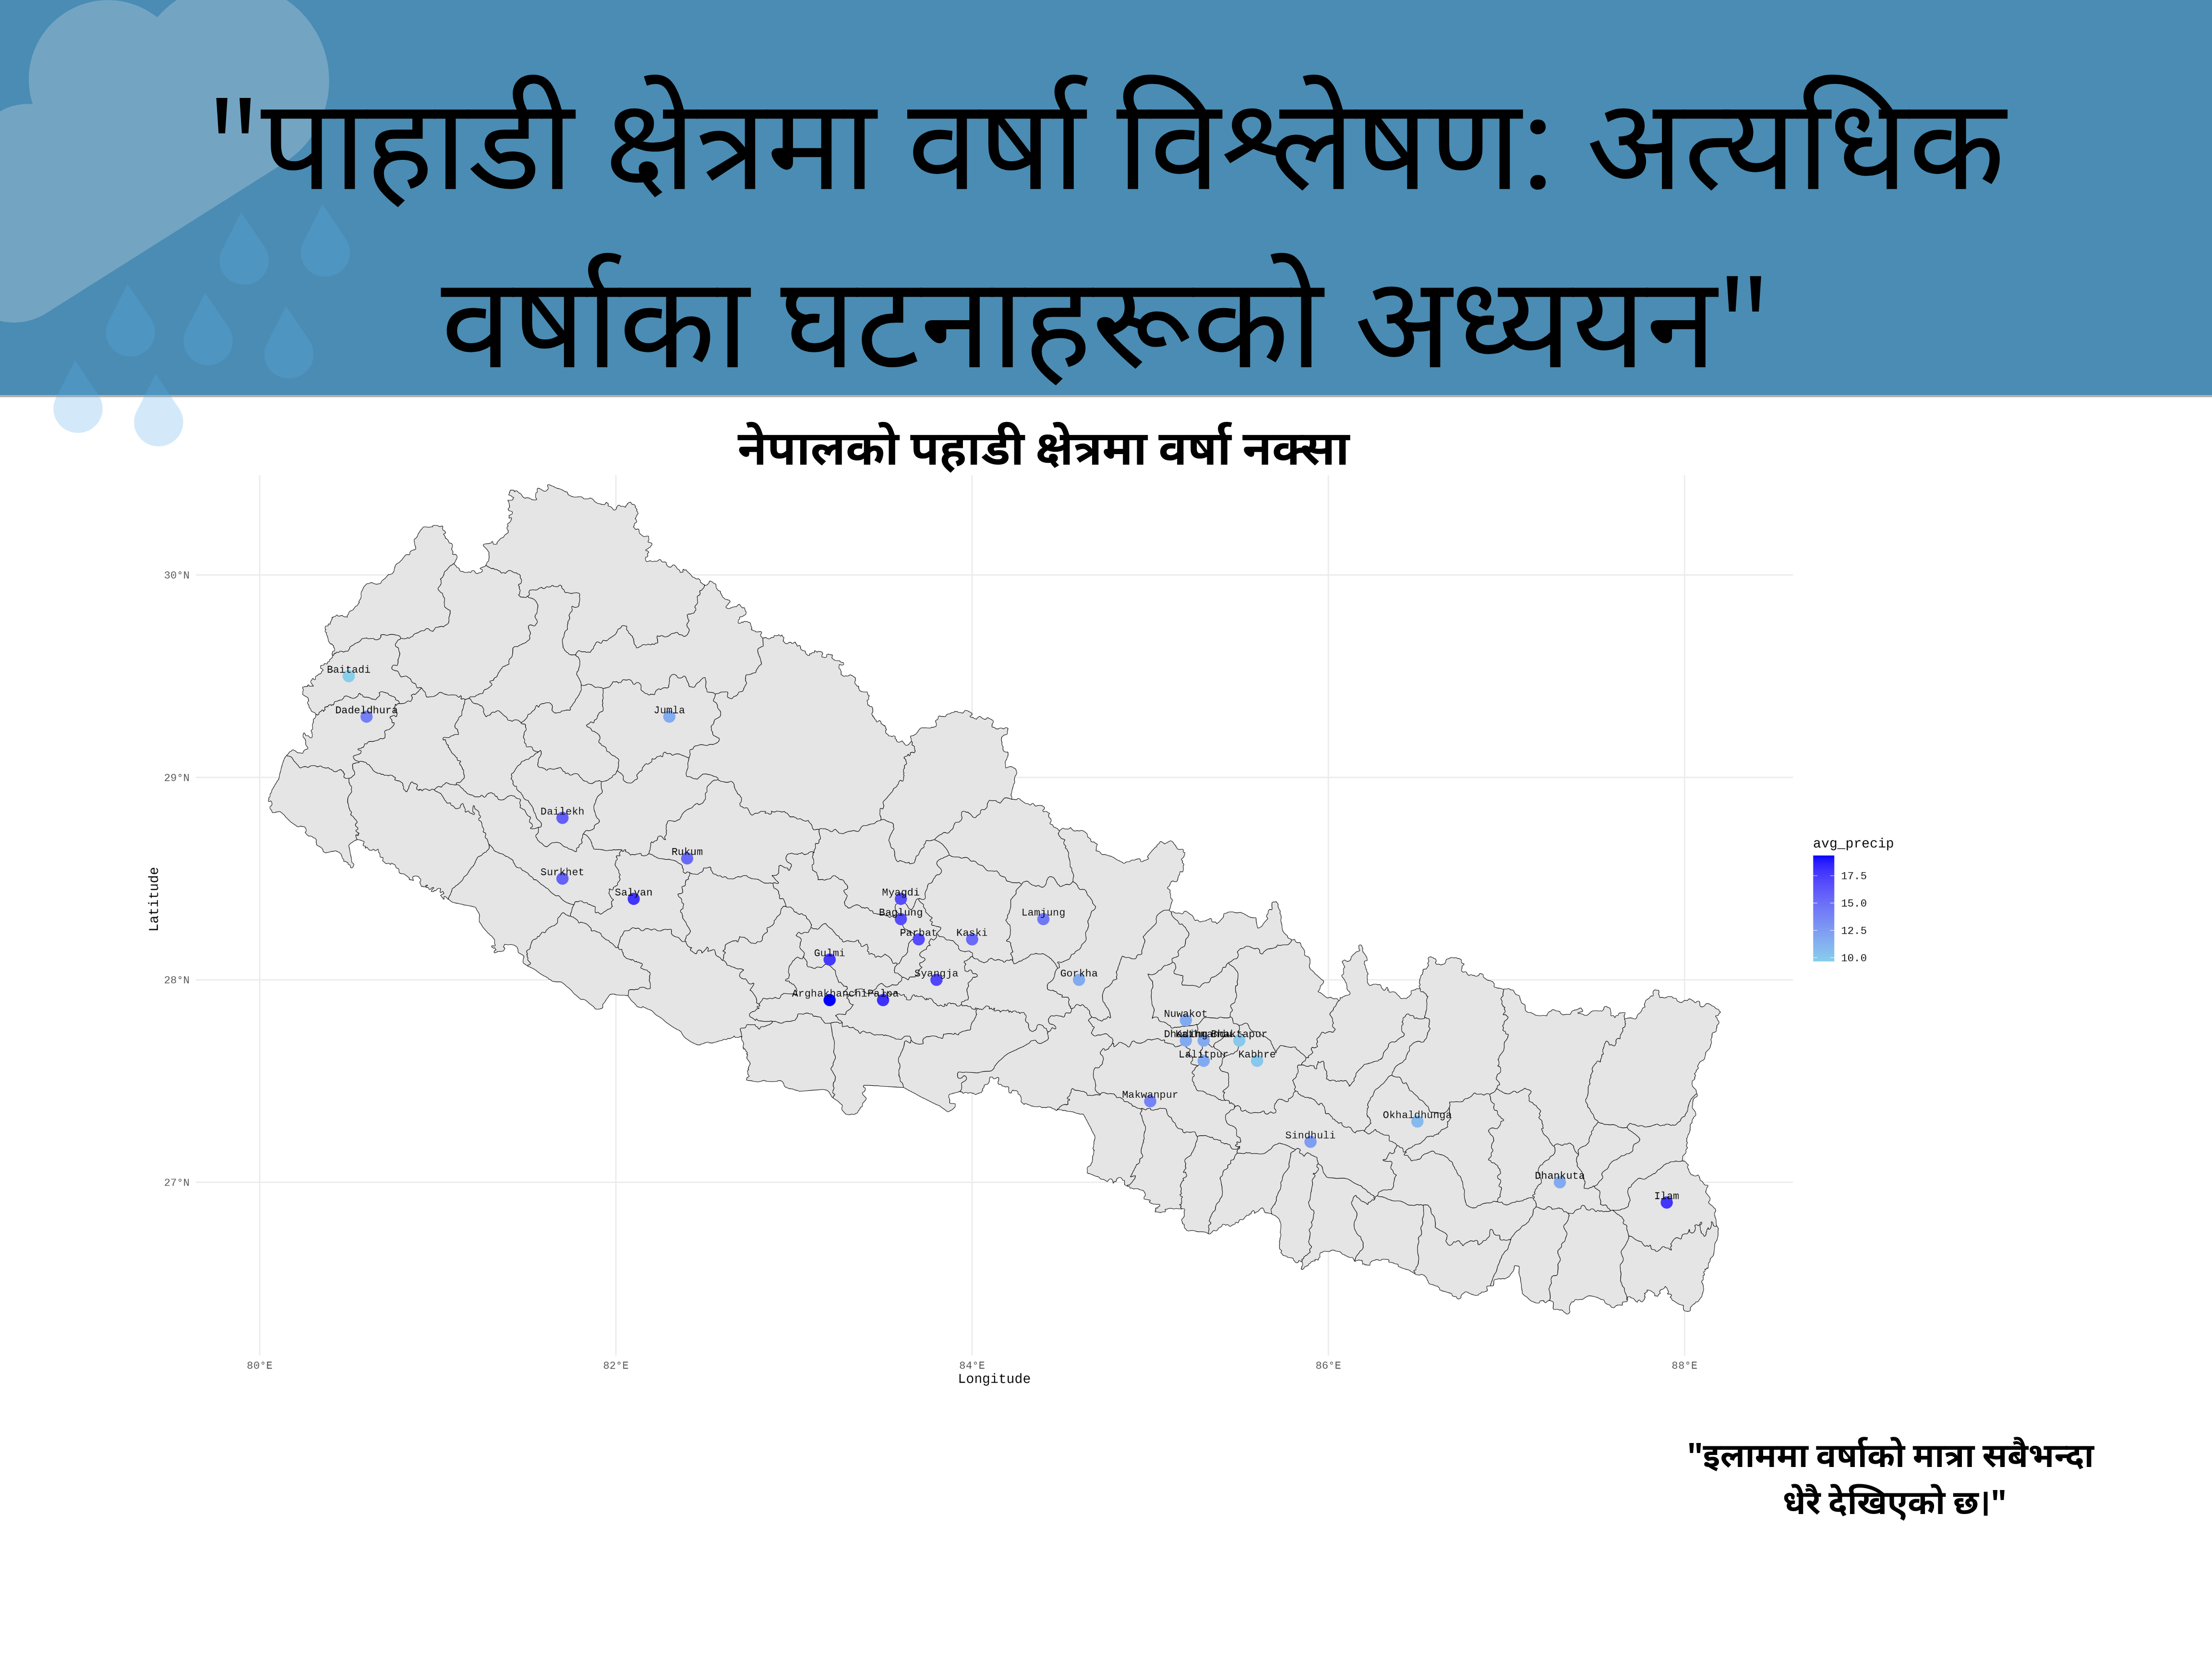
\includegraphics[width=0.7\textwidth]{figures/info1.png}
\end{figure}

\begin{figure}[h]
\centering
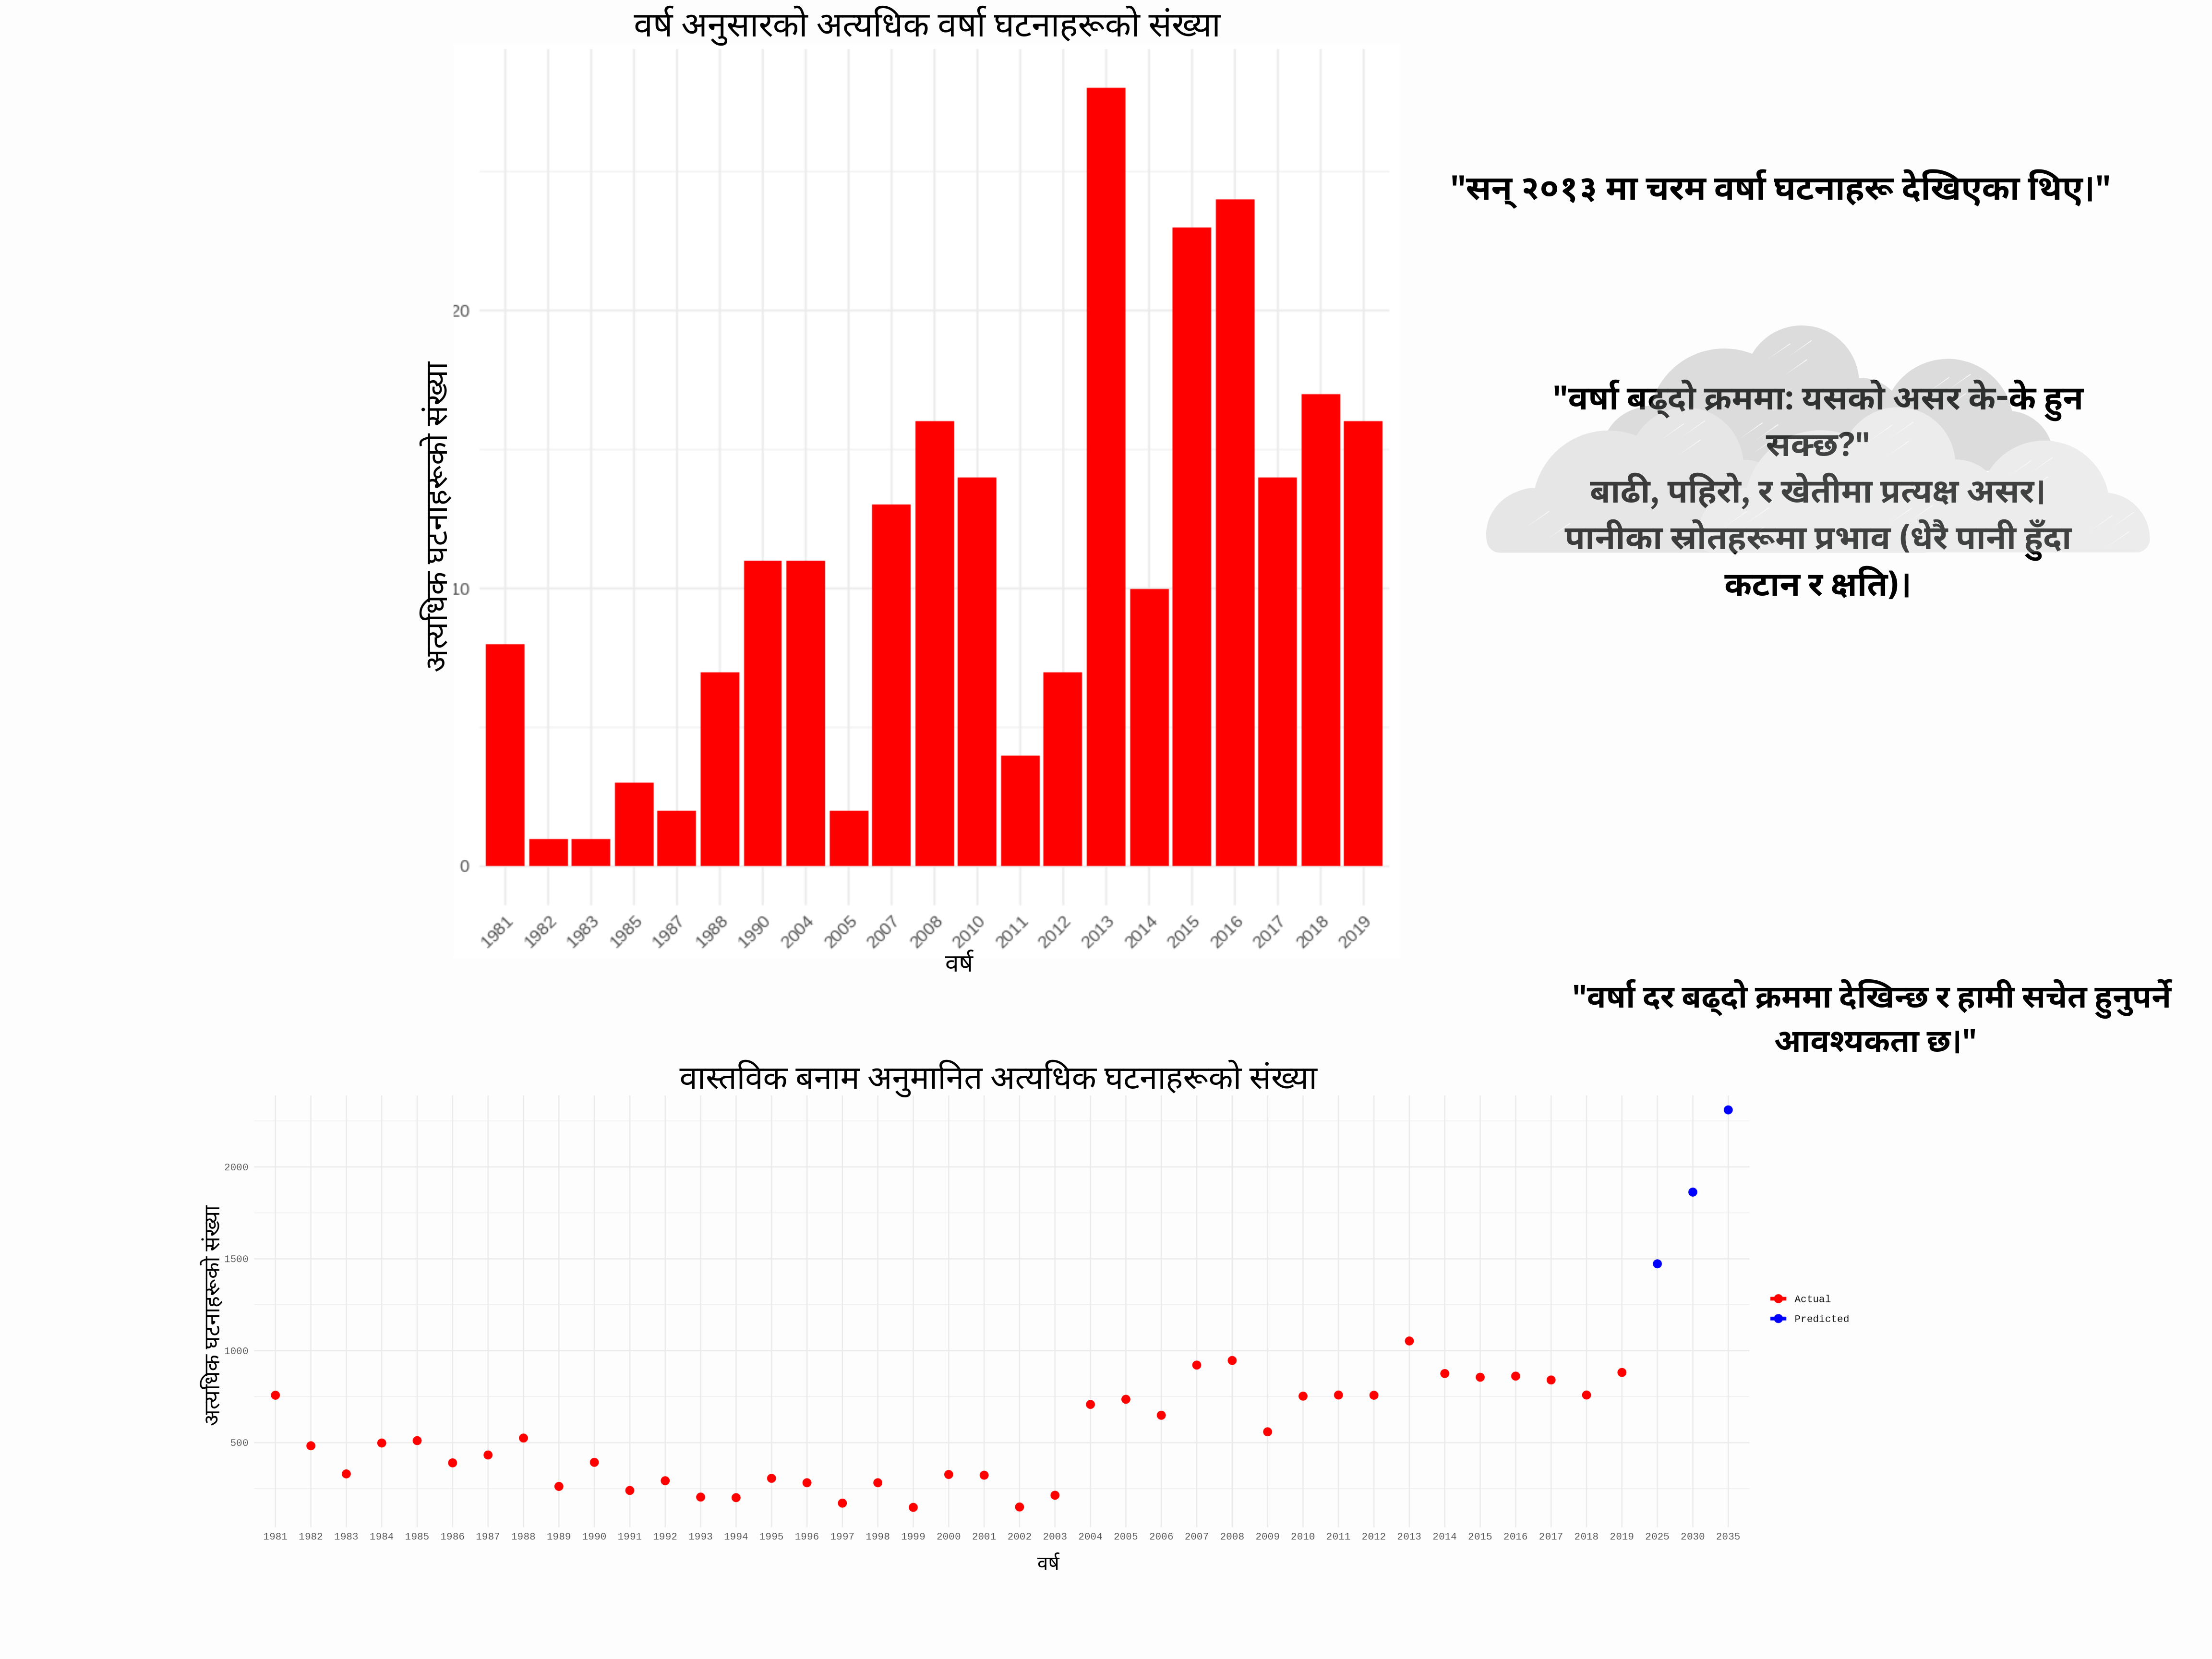
\includegraphics[width=0.7\textwidth]{figures/info2.png}
\caption{Figure 7.1: Infographic Poster}
\end{figure}

\clearpage
\section{Dashboard Using R}

\subsection*{Why Dashboards?}
A dashboard acts like a control panel for your data, showing the most important trends and statistics at a glance. In climate data analysis, dashboards can help track real-time changes in temperature, humidity, or rainfall and communicate findings visually.

\subsection*{Creating a Climate Dashboard with R}
Creating a visual and interactive dashboard is an excellent way to explore and communicate insights from climate data. In this section, we will walk through how to create a climate dashboard using \texttt{flexdashboard}, \texttt{ggplot2}, and \texttt{lubridate} packages in R.

\subsubsection*{1. Installing Required Packages}
Before proceeding, ensure the necessary packages are installed. Run the following commands in your R console:
\begin{verbatim}
install.packages("ggplot2") 
install.packages("flexdashboard") 
install.packages("lubridate")
\end{verbatim}

These packages serve the following purposes:
\begin{itemize}
    \item \textbf{ggplot2} — for creating advanced visualizations.
    \item \textbf{flexdashboard} — for building dashboards using R Markdown.
    \item \textbf{lubridate} — for handling and manipulating date-time data.
\end{itemize}

\subsubsection*{2. Loading Your Climate Dataset}
Prepare your dataset in CSV format. Suppose the file is named \texttt{dataframe.csv}. Load it into R using:

\begin{verbatim}
climate_data <- read.csv("dataframe.csv")
\end{verbatim}

This command reads the CSV file and stores it in the object \texttt{climate\_data}, which we will use for visualization.

\subsubsection*{3. Creating the FlexDashboard File}
\begin{enumerate}
  \item Open Visual Studio Code (VSCode) or RStudio. 
  \item Create a new file named \texttt{dashboard.Rmd}.

  \item At the top of the file, include the following YAML header:

\begin{verbatim}
---
title: "My Climate Data Dashboard"
output: 
  flexdashboard::flex_dashboard
runtime: shiny
---
\end{verbatim}
\end{enumerate}
This YAML header defines the document title, output format, and specifies that the dashboard will have interactive capabilities using Shiny.

\subsubsection*{4. Adding Plots to the Dashboard}

Use R code chunks within the R Markdown file to include visualizations. Here’s how you can organize two plots in the first row of your dashboard:

\textbf{Row 1: Temperature Histogram (Left) and Precipitation Bar Plot (Right)}

\begin{verbatim}
```{r}

# Left Column: Temperature Histogram

ggplot(climate_data, aes(x =Temp_2m)) +
geom_histogram(binwidth =1, fill ="skyblue",color ="black",alpha = 0.7)+
labs(
  title ="Temperature Histogram", 
  x = "Temperature (°C)", 
  y ="Density")+
  theme_minimal()

# Right Column: Precipitation Histogram

ggplot(climate_data, aes(x = Precip)) +
geom_histogram(binwidth =1,fill ="skyblue",color ="black",alpha = 0.7)+
labs(
  title = "Precipitation Histogram",
  x ="Precipitation",
  y = "Density")+
  theme_minimal()

\end{verbatim}

\subsubsection*{5. Rendering the Dashboard}
\begin{enumerate}
\item Once you have completed your \texttt{.Rmd} file with all necessary code chunks:
\item Save the file.
\item Render it in the R terminal by typing:
\begin{verbatim}
rmarkdown::render('d:/R project/dashboard.Rmd')
\end{verbatim}
\end{enumerate}

This will generate an HTML output of the dashboard.

\subsubsection*{6. Viewing the Dashboard}
Navigate to the location where the HTML file is saved. Open it using any web browser. You should see an interactive dashboard displaying the plots you’ve created.

% Figure here--------------------------
\begin{figure}[h]
\centering
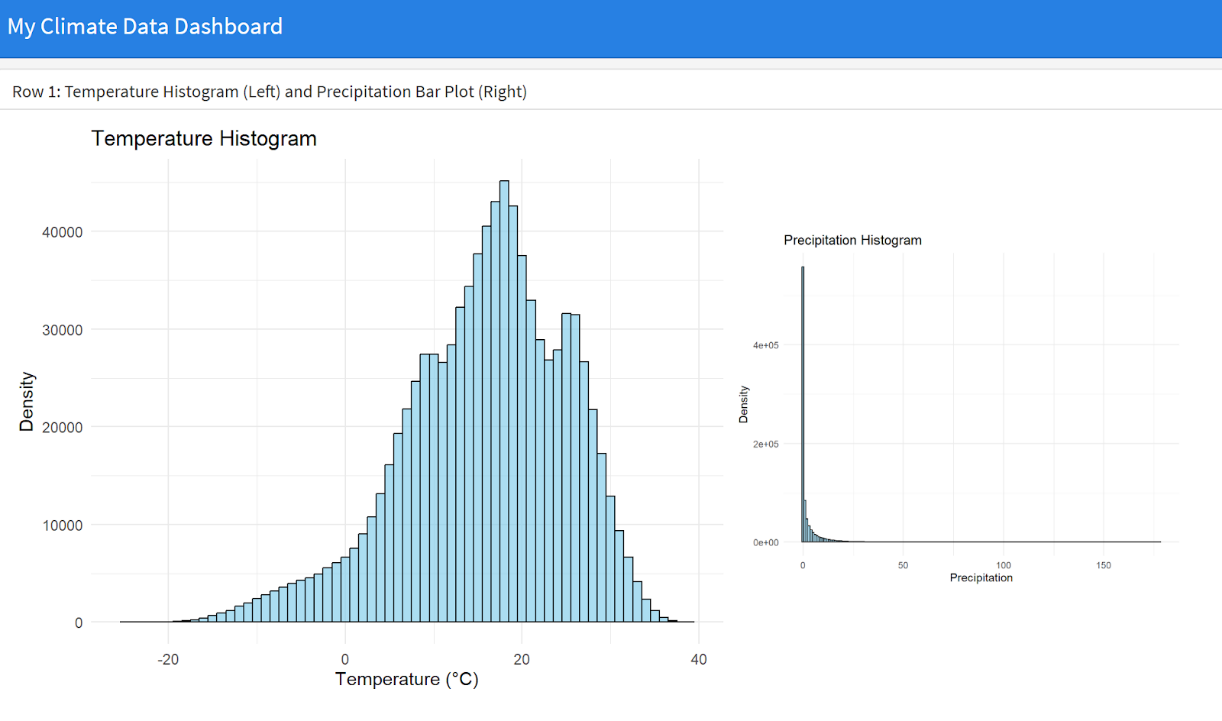
\includegraphics[width=0.8\textwidth]{figures/dashboard.png}
\caption{Figure 7.2: Dashboard using R}
\end{figure}

\subsection*{Summary Checklist for Learners}
\begin{itemize}
\item Installed required packages (\texttt{ggplot2}, \texttt{flexdashboard}, \texttt{lubridate})
\item Loaded and verified climate data
\item Created an R Markdown file with the correct YAML header
\item Added at least two informative visualizations
\item Rendered and opened the dashboard
\end{itemize}

\subsection*{Next Steps}
Try adding more components such as:
\begin{itemize}
\item Time series plots for temperature trends.
\item Interactive filters using Shiny widgets.
\item Value boxes showing summary statistics.
\end{itemize}
